%% ggf:
% \part{Appendix}
% \label{part:appendix}

\chapter{Implementation Details}

\section{Determining the Lexical Scope}
\label{sec:app_lexical_scope}
In this section, we describe in more detail how \msname determines the collection of enclosing classes which is necessary for generating a \texttt{LexicalScope} instance for the keywords \texttt{outer} and \texttt{scope}. The system has to traverse the meta model. It is not sufficient to simply return the collection \texttt{\{ enclosing. enclosing enclosing. enclosing enclosing enclosing. ... \}}. For example, in Figure~\ref{fig:app_cls_diagr}, \texttt{C} is a class extension whose target class is \texttt{D}. \texttt{B} is a class extension whose target class is \texttt{G}. Therefore, in \texttt{foo}, \texttt{enclosing} is \texttt{B} (which is the same class object as \texttt{G}) and \texttt{enclosing enclosing} is \texttt{H}, because \texttt{G enclosing} is \texttt{H}.

\begin{figure}[!htp]
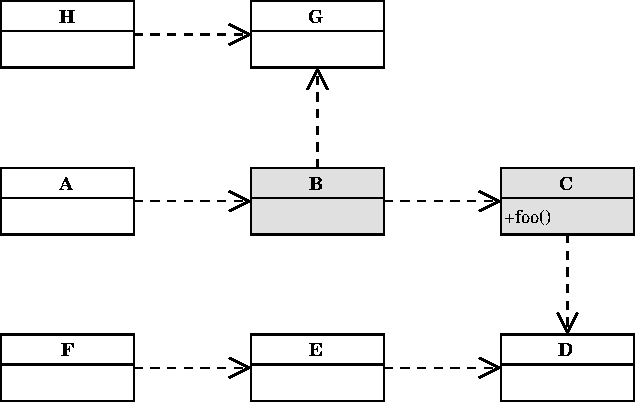
\includegraphics[width=0.75\textwidth]{app_cls_diagr.pdf}
\centering
\caption[Example: Nested classes with class extensions]{Example: Nested classes with class extensions. All gray classes are class extensions. Horizontal arrows indicate \emph{class nesting}. Vertical arrows indicate \emph{target class references}.}
\label{fig:app_cls_diagr}
\end{figure}

Figure~\ref{fig:app_lex_scope} shows the relevant parts of the meta model for determining the lexical scope of \texttt{foo}. Every class specification has a reference to its meta class specification and vice versa. For every class specification, there is a corresponding corresponding method specification holding the class cache and the \texttt{instantiations} dictionary which also acts as the argument cache (see Section~\ref{sec:impl_migration}).

\begin{figure}[!htp]
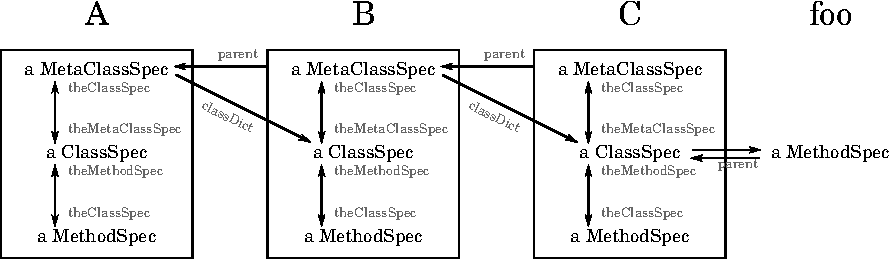
\includegraphics[width=\textwidth]{lexical_scope_app_ex.pdf}
\caption[Example: Detailed meta model]{Example: Detailed meta model. Class \texttt{B} is nested within class \texttt{A} and class \texttt{C} is nested within class \texttt{B}. \texttt{foo} is an instance method of class \texttt{C}. All three entities within a box have the same meta class specification as a parent.}
\label{fig:app_lex_scope}
\end{figure}

Figure~\ref{fig:app_det_lex_scope_algo} shows the algorithm for determining the lexical scope, given that a method specification (\texttt{foo}) is instantitated within the target class \texttt{cls}. The first enclosing class should be \texttt{B}. \texttt{B}'s meta class specification can be reached by following the parent pointer twice. However, we do not need the specification but the actual class object of \texttt{B}. The \texttt{instantiations} dictionary maps class specification instantiations (e.g. the class object \texttt{C} which is the target class \texttt{cls}) to an array of the enclosing class object and the arguments provided to the class accessor method\footnote{Note, that \texttt{instantiations} can contain multiple class specification instantiations in case the class in question is an extended inherited nested class which was not subclassed or a paramterized class.}. The enclosing class object is always the first element in that array. Therefore, the first enclosing class in the lexical scope of \texttt{foo} is the first element in the \texttt{instantiations} array of \texttt{self parent parent theClassSpec theMethodSpec}.

\begin{figure}[!htp]
\begin{lstlisting}
<@\textbf{MethodSpecification>>lexicalScopeIn:}@> cls
    <@\textcolor{gray}{| enclosingClasses currentCls currentMetaClassSpec |}@>
    <@\textcolor{gray}{enclosingClasses}@> := OrderedCollection new.
    <@\textcolor{gray}{currentCls}@> := cls.
    <@\textcolor{gray}{currentMetaClassSpec}@> := self parent parent.

    <@\textcolor{gray}{enclosingClasses}@> add: (<@\textcolor{gray}{currentCls}@> := 
        (<@\textcolor{gray}{currentMetaClassSpec}@> theClassSpec theMethodSpec 
            instantiations at: <@\textcolor{gray}{currentCls}@>) first).

    [ <@\textcolor{gray}{currentMetaClassSpec}@> parent isNil ] whileFalse: [
        <@\textcolor{gray}{currentMetaClassSpec}@> := <@\textcolor{gray}{currentMetaClassSpec}@> parent.
        <@\textcolor{gray}{enclosingClasses}@> add: (<@\textcolor{gray}{currentCls}@> := 
            (<@\textcolor{gray}{currentMetaClassSpec}@> theClassSpec theMethodSpec 
                instantiations at: <@\textcolor{gray}{currentCls}@>) first) ].

    ^ <@\textcolor{gray}{enclosingClasses}@>
\end{lstlisting}
\caption[Algorithm: Determining the lexical scope of a method]{Algorithm: Determining all enclosing classes in the lexical scope of a method.}
\label{fig:app_det_lex_scope_algo}
\end{figure}

The next enclosing classes can be found by following the parent relationship and using the previously-found enclosing class as a key in the next \texttt{instantiations} dictionary.

\section{Traits}
\label{sec:app_traits}
In Section~\ref{sec:use_cases_traits}, we gave an overview of how traits can be implemented with nested classes and include hooks, but did not describe how to invoke a trait method within the resolution code of a conflicting method.

In \msname, traits are implemented as mixins, which are wrapped in unparameterized classes (\emph{unparameterized class generator pattern}, see Section~\ref{sec:usecase_classgen}). Figure~\ref{fig:algo_trait_res} shows how trait methods can be invoked. The programmer has to call the method \texttt{trait:perform:withArguments:} and has to provide the trait (i.e., the unparameterized class generator), the message symbol, and a collection of arguments. \msname then goes through all superclasses of the receiver, in order to find the mixed-in trait. \texttt{ProtoObject} provides a functionality which can then be used to execute the corresponding \texttt{CompiledMethod} object in the context of \texttt{self}.

\begin{figure}[!htp]
\begin{lstlisting}
<@\textbf{Object>>trait:}@> classGenerator <@\textbf{perform:}@> symbol <@\textbf{withArguments:}@> args
    <@\textcolor{gray}{| trait |}@>
    <@\textcolor{gray}{trait}@> := self class allSuperclasses detect: [ <@\textcolor{gray}{:cls}@> |
        <@\textcolor{gray}{cls}@> specification includes: 
            (classGenerator specification classAt: #Mixin:) ].
    ^ self withArgs: args executeMethod: <@\textcolor{gray}{trait}@>>>symbol
\end{lstlisting}
\caption[Algorithm: Resolving trait conflicts]{Algorithm: Resolving trait conflicts. This method can be used to invoke a method implementation in a specific trait.}
\label{fig:algo_trait_res}
\end{figure}

Note, that it is important to lookup the mixed-in trait in the superclass hierarchy of the receiver. Every mixed-in trait (\emph{trait instantiation}) provides the same methods, but whenever instance variables are accessed, the bytecode of two instantiations of the same trait method can differ (see Section~\ref{sec:impl_ch_inst_cl_vars}).

%%% Local Variables: 
%%% mode: latex
%%% End: 
